\titleformat{\chapter}[display]{\bfseries\centering}{\huge Chapter \thechapter}{1em}{\Huge #1}
\newgeometry{top=3cm, bottom=2.2cm, left=3cm, right=2cm, headsep=1.2cm, footskip=1cm, headheight=0.3cm, textheight=24.5cm, textwidth=16cm}
\onehalfspacing

\pagestyle{fancy}
\fancyhf{}
\renewcommand{\headrulewidth}{0pt}
\lhead{Chapter 1}
\rhead{Introduction}
\cfoot{\thepage}
\chapter{Introduction}

\section{Introduction}
\noindent Social media is full of useful messages: job offers, college notices, bank alerts and chats with friends. The same channels are also used to cheat and hurt people. A fake internship may ask for a ``registration fee'' or an OTP, a link may copy a real login page, an account may be a bot, and a chat may contain threats or bullying. Most protection today comes from platform moderation and user reports, which is slow and rarely explains anything.\\

\noindent \textbf{Sentinel} is a safety assistant that runs on the user's own computer. The user pastes a message, a link, a chat or an account, or switches on \emph{auto-scan} in the Chrome extension, and Sentinel tells them three things for each kind of threat: what it found, what it could not check, and what to do next. It never calls an unknown link ``safe'' or an unusual account ``fake''. The project has two parts: a working application, and a research pipeline that trains and tests machine-learning (ML) models. A model is added to the application only if it passes a test that was fixed before training. This report covers the work done in Semester VII.

\section{Background: Key Terms}
\begin{itemize}
\item \textbf{Phishing / smishing:} messages that trick people into giving passwords, OTPs or money, usually through a fake website link (smishing: by SMS or chat).
\item \textbf{Social bot / fake account:} an account run by a program, or one that pretends to be someone else \cite{lit3}.
\item \textbf{Harmful language:} threats, bullying, hate and messages about self-harm. Context matters: a quoted insult is not the same as a direct one \cite{cad}.
\item \textbf{Punycode:} a way of writing non-English web addresses (\texttt{xn--}); it can make a fake site look like a real one \cite{homograph}.
\item \textbf{TF-IDF, logistic regression, gradient boosting:} standard ways of turning text into numbers and classifying it \cite{sklearn}. \textbf{DistilBERT} is a small, fast language model \cite{distilbert}.
\item \textbf{Calibration:} adjusting a model's scores so that ``90\%'' really means right about 90\% of the time \cite{guo}.
\item \textbf{MinHash:} a short ``fingerprint'' of a text that lets two similar messages be matched without storing the text \cite{broder}.
\item \textbf{$k$-anonymity:} sharing something only when at least $k$ different people report it, so no single person can be identified \cite{sweeney}.
\item \textbf{Data leakage:} when near-copies of the same item end up in both training and test data, making a model look better than it is.
\item \textbf{Manifest V3 and HMAC:} the current Chrome extension system \cite{mv3}, and a signed checksum that proves data was not changed \cite{hmac}.
\end{itemize}

\section{Challenges}
\begin{itemize}
\item \textbf{Threats come together:} one post can contain a scam message, a fake link and a fake account at the same time.
\item \textbf{Users see only part of the picture:} an ordinary user cannot see login logs or full posting histories, so many research methods \cite{lit2} cannot be used.
\item \textbf{Mixed and disguised language:} Indian users write in English and Hinglish, and abusers hide words (\texttt{1d10t}, \texttt{k.y.s}, \texttt{stuuupid}).
\item \textbf{High scores can mislead:} a model can score 97\% on a biased dataset and still fail on real messages.
\item \textbf{Privacy and platform rules:} messages are private, and scraping profiles breaks platform terms.
\item \textbf{Limited hardware:} the models must run on a normal laptop CPU.
\end{itemize}

\section{Motivation}
\noindent Students are common targets of fake internships, fake college or bank portals and online bullying. Existing tools handle one threat at a time and give a verdict without a reason. We wanted a tool a student can use before replying to a suspicious message: it runs locally, covers the common threats, explains itself and is honest about what it cannot check.

\section{Problem Statement and Proposed Solution}
\noindent\textbf{Problem statement.} Social media users face scam messages, phishing links, harmful language and fake accounts. Current protection depends on manual moderation or separate tools that do not explain their decisions. A system is needed that checks what the user can see, using rules, machine learning and natural language processing (NLP), without sending their data away or overstating its certainty.\\

\noindent\textbf{Objectives.}
\begin{enumerate}
\item Let a user check a message, link, chat, profile or account from a web app or a Chrome extension, with no cloud account.
\item Report each kind of threat separately, with evidence, missing checks and a next step.
\item Detect harmful language in English and Hinglish, and give support numbers for self-harm.
\item Warn users while they browse, only on sites they choose.
\item Estimate whether an account is a bot using only official APIs or data the user provides.
\item Let users warn each other about new scams without sharing message text.
\item Release a learned model only after it passes a fair test on data it has never seen.
\end{enumerate}

\noindent\textbf{Proposed solution.} Sentinel is a small Python server on the user's computer (address 127.0.0.1), used by a four-page web app and a Chrome extension. Each request goes through separate checkers: fraud rules, harm rules, a learned scam-text model, a community scam matcher, profile checks and bot detection. Figure~\ref{fig:block} shows the overall design.

\begin{figure}[H]
\centering
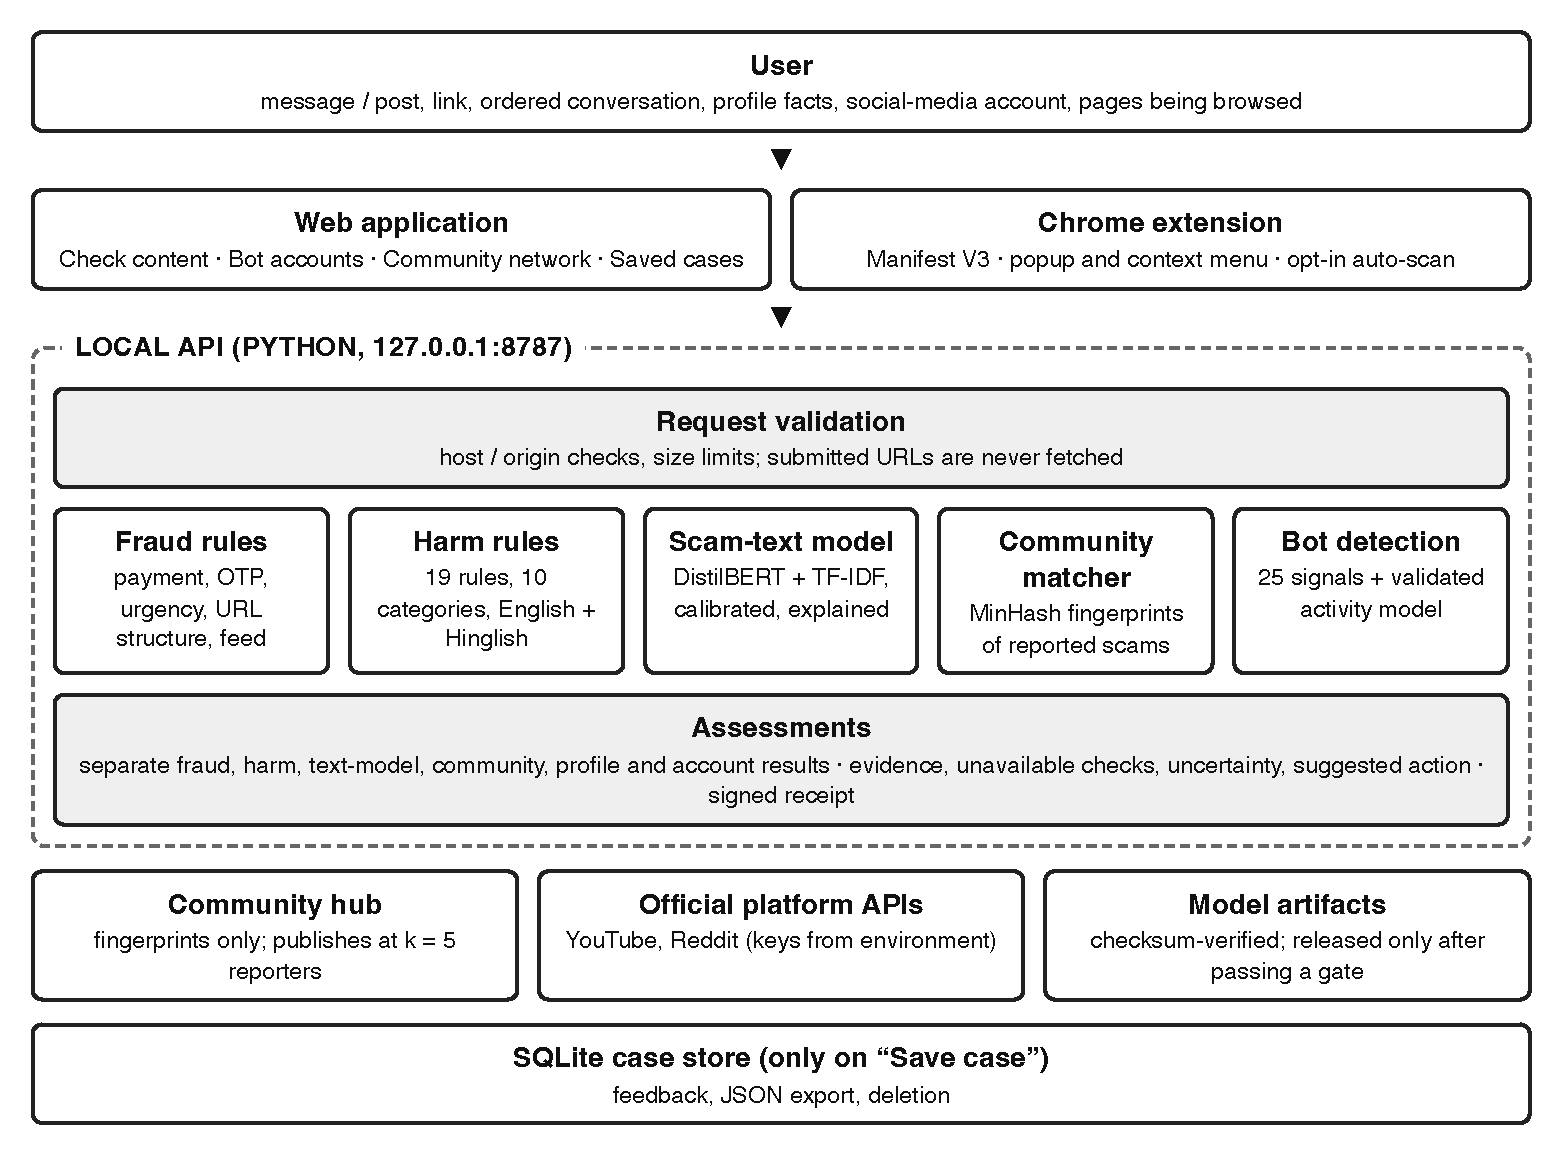
\includegraphics[width=0.8\linewidth]{dia2/block_v2.pdf}
\caption{General block diagram of Sentinel}
\label{fig:block}
\end{figure}

\noindent\textbf{Organization of the report.} Chapter 2 reviews existing work, Chapter 3 describes the design, Chapter 4 the plan and test setup, Chapter 5 the results, Chapter 6 the conclusion and Chapter 7 the references.
